\scanpage{20}nier (ou, ce qui revient au même, $c$) est bien déterminée. Les unipotents qui définissent ladite filtration, en termes d'un $i$ qui la définit, sont
% Typed interlinear addition and its connected handwritten curved leader.
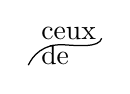
\begin{tikzpicture}[baseline=(de.base),x=1em,y=1ex]
\node[anchor=base west,inner sep=0pt] (de) at (0,0) {de};
\node[anchor=base west,inner sep=0pt] at (0,2.05) {\inserted{ceux}};
\draw[line width=.45pt] (-.45,-.10) .. controls (-.28,.75) and (.08,1.65) .. (.78,1.62) .. controls (1.32,1.55) and (2.12,1.34) .. (2.20,2.16);
\end{tikzpicture}
la forme $\exp(e)$, où $e$ parcourt $\handwritten{\unsure{\mathfrak{g}|\mathscr{G}}}(2)^{\handwritten{*}}+\operatorname{Fil}^{\handwritten{3}}(\handwritten{\mathfrak{g}})$. Ils forment une classe de conjugaison d'éléments de $U$ \uline{par} $P$ (NB mais pas par $U$), les classes de conjugaison \uline{par} $U$ s'identifiant aux ensembles de la forme $(\exp(e)\handwritten{\mid}e\handwritten{\in}a+\operatorname{Fil}^{\handwritten{3}}(\handwritten{\mathfrak{g}}\unsure{.|,}))$, où $a\handwritten{\in\mathfrak{g}}(2)^{\handwritten{*}}$ est un élément quelconque.\deleted{de}

\uline{Cas principal}. Pour qu'on ait\hspace{1.5em}$(1)=0$, il faut et suffit que \deleted{l'homomor} la classe d'homomorphismes $f:\operatorname{Sl}(2,k)\hspace{1.5em}G$ envisagée soit ``princi%
% Each of these two cells has p and a contours; their chronological order is unresolved.
\unsure{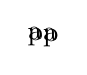
\begin{tikzpicture}[baseline=(pa.base),x=1em,y=1ex]
\node[anchor=base west,inner sep=0pt] (pa) at (0,0) {p};
\node[anchor=base west,inner sep=0pt] at (.02,.10) {a};
\node[anchor=base west,inner sep=0pt] at (.56,0) {a};
\node[anchor=base west,inner sep=0pt] at (.56,-.05) {p};
\end{tikzpicture}}%
le'' au sens de Dynkin-Kostant. Alors le parabolique associé $P$ est un Borel (la réciproque n'étant pas vraie \deleted{sans doute}, cf table de Dynkin), et le groupe $Z_o$ est le groupe unité (i.e. $\operatorname{Dyn}_c$ est un torseur sous $G$),
% The first cell has an l-like upright plus opposed loops and lower extensions.
% The extra contour is reproduced without assigning a predecessor or chronology.
\unsure{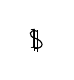
\begin{tikzpicture}[baseline=(ell.base),x=1em,y=1ex]
\node[anchor=base west,inner sep=0pt] (ell) at (0,0) {l};
\draw[line width=.40pt] (.29,1.48) .. controls (-.04,1.74) and (-.05,1.02) .. (.19,.91) .. controls (.53,.65) and (.55,.02) .. (.16,.04);
\draw[line width=.30pt] (.18,1.63) -- (.18,-.20);
\draw[line width=.30pt] (.29,1.58) -- (.29,-.22);
\end{tikzpicture}}a réciproque n'étant pas vraie sans doute.
\margin{\handwritten{\uline{ex}\quad Cas $A_2,A_4$ les paraboliques associés aux \unsure{unipotents} ``sous-réguliers'' sont des \unsure{borels|Borels} !}}
% slanted margin note, at the lower left beside the Cas principal paragraph
% archive sheet number: 19
